%!TEX root = ../main.tex

\par
I perform two major experiments to analyze the efficacy.
First, I need to determine the underlying dimensionality of the vector space the hurricanes lie in.
To do this, I try embedding a subset of the full dataset into $\R^{i}$ for $i=1,\ldots,15$, and then regressing the Nardaraya-Watson estimator for each case.
I then predict a different subset of the data to evaluate the accuracy of the model, for each number of dimensions.
In Figure~\ref{fig:dimensions}, I plot the accuracy by the number of dimensions $i$.
In Figure~\ref{fig:confident_dimensions}, I plot the accuracy (but this time only including points for which the estimator has at least $90\%$ confidence) by the number of dimensions.
The overall accuracy is roughly improving up to $i=15$, but not after.
On the other hand, the accuracy for high confidence points appears to be optimal at $i=10$.
This makes it difficult to judge the underlying dimension of the data, so I will experiment with both choices of dimension.

\begin{figure*}
	\centering
	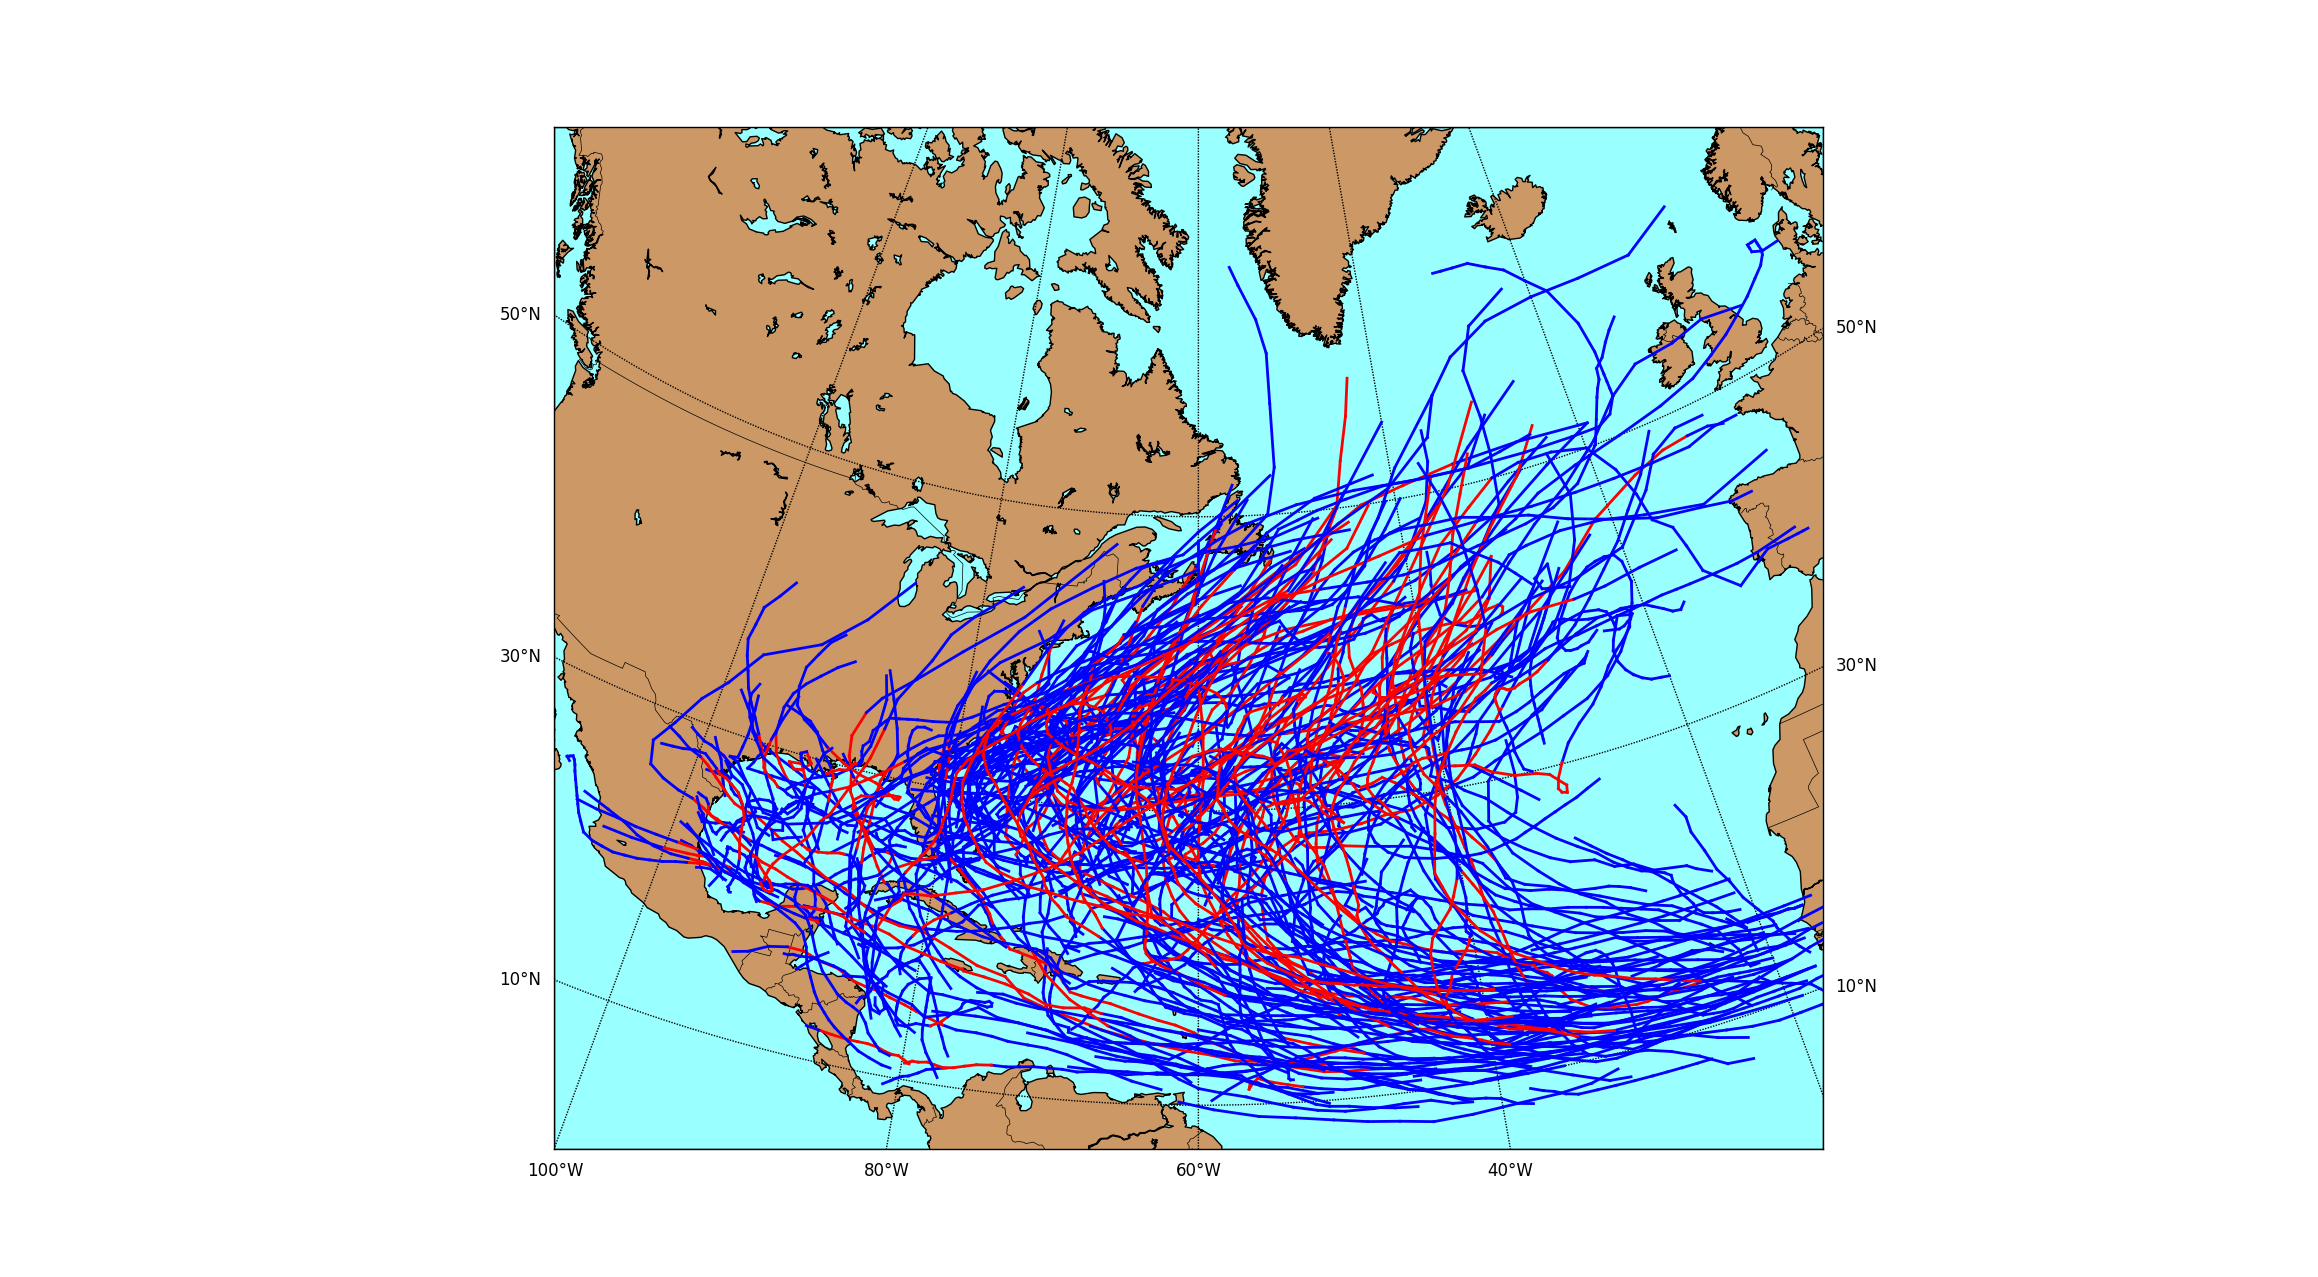
\includegraphics[width=\textwidth]{images/got_it_right.png}
	\caption{A plot of all hurricanes successfully predicted by the dimension-$15$ model.}
	\label{fig:got_it_right}
\end{figure*}

\begin{figure*}
	\centering
	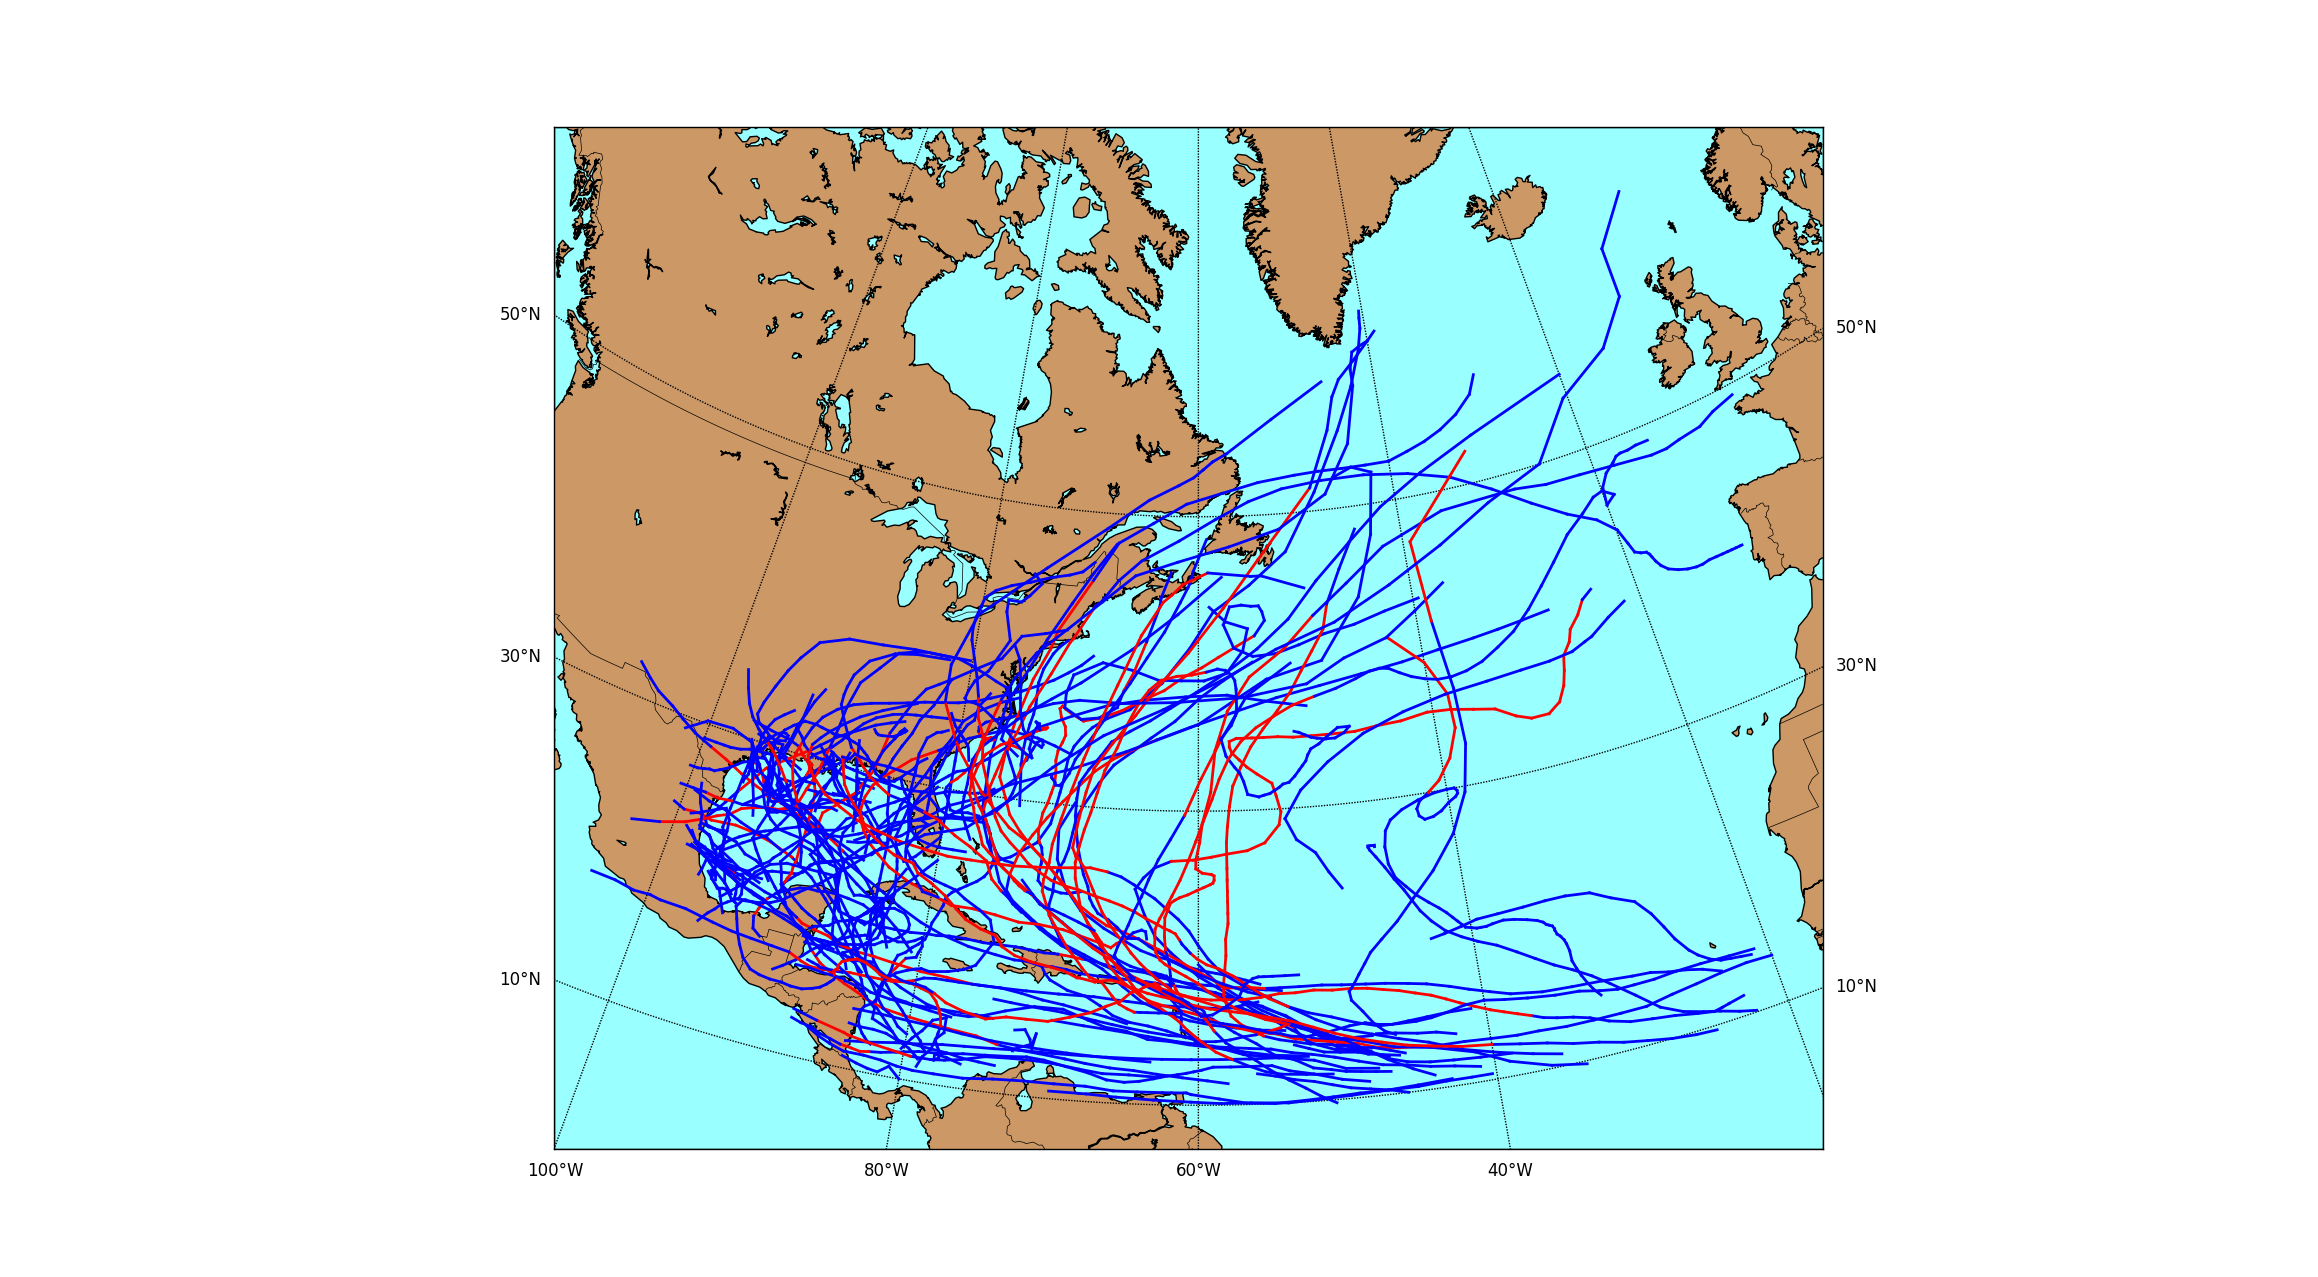
\includegraphics[width=\textwidth]{images/got_it_wrong.png}
	\caption{A plot of all hurricanes not successfully predicted by the dimension-$15$ model.}
	\label{fig:got_it_wrong}
\end{figure*}

\par
First, I will test with $i=10$.
In order to fully evaluate how accurate my algorithm is, I train it on every huurricane from 2000 through 2018, and then test it on every hurricane from 1970 through 1999.
Out of $479$ hurricanes in the test dataset, the learned model correctly predicts $344$; this is an accuracy of $0.72$.

\par
Now, I will test with $i=15$.
In order to fully evaluate how accurate my algorithm is, I train it on every huurricane from 2000 through 2018, and then test it on every hurricane from 1970 through 1999.
Out of $479$ hurricanes in the test dataset, the learned model correctly predicts $335$; this is an accuracy of $0.70$.

\par
Additionally, in the case where $i=15$, I plot all of the successfully predicted storms in Figure~\ref{fig:got_it_right}, and all of the not successfully predicted storms in Figure~\ref{fig:got_it_wrong}.
There's a clear trend -- storms further to the north are significantly easier to predict in the early stages of their lifetime just using statistics, whereas storms further to the south and in the Gulf of Mexico are more challenging.